\documentclass[a4paper]{article}
\usepackage{Sweave}
\usepackage{lscape}
\usepackage{color}
\usepackage{colordvi}
\usepackage{graphicx}
\usepackage[round]{natbib}

\title{Nonparametric maximum likelihood estimation for random effect models in R\\
\vspace{1cm}
\large Vignette to R package {\bf npmlreg}}
\vspace{2cm}
\author{Jochen Einbeck and John Hinde}


%  in R:
%  library(utils)  % Sweave
%  Sweave("npml-R2.Stex")
%  in WinEdit:
%  latex npml-R2.tex
%  in R:
%  Stangle("npmlreg.Stex")
%\VignetteIndexEntry{NPML estimation for random effect models in R} 
%\VignetteDepends{npmlreg, MASS, gamlss, forward, nlme}
%\VignetteKeyword{NPML}


\begin{document}
\begin{landscape}
\pagestyle{plain}


\maketitle
\thispagestyle{empty}


\newpage
\tableofcontents

\newpage

\section{Introduction}

Nonparametric maximum likelihood (NPML) estimation is an attractive tool for the fitting 
of generalized linear models with random effects, 
which can be considered as a special case of generalized linear mixed models (GLMMs).  
One crucial advantage of the NPML approach is that the random effect distribution does not need 
to be specified a priori, whereas the huge body of literature on GLMMs restricts nearly exclusively 
on normally distributed random effects. Further, complicated integrations are avoided by approxmating 
the marginal likelihood by a simple finite mixture, for which standard fitting algorithms based on EM 
exist and can be applied. NPML for generalized linear models with random effects was previously implemented 
by Aitkin \& Francis (1995) in the GLIM4 language, which is however no longer widely used. The main functions 
of this package,  {\tt alldist}  (for overdispersion) and {\tt allvc} (for variance component models), 
are  modified and extended versions of their homonymous counterparts in GLIM4, and have been translated 
to R originally by Ross Darnell.



In this handbook the concept of NPML estimation is briefly explained (Section \ref{method}) and
 a variety of  data examples are given (Section \ref{examples}), which illustrate the functionalities 
 of {\tt alldist} and {\tt allvc}. The  R package {\bf npmlreg} is available for download on CRAN at
\begin{center}
{\tt http://cran.r-project.org}.
\end{center}

 
\vspace{0.3cm}
{\em Key Words:}
 Varying coefficient models, random effect models, mixed models, mixture models,  Gaussian Quadrature, EM algorithm, Two-level models,
 exponential family regression models.
   

\section{Random effect modelling with exponential family mixtures}\label{method}


Assume there is given a set of explanatory vectors $x_1, \ldots,
x_n$ and a set of observations  $y_1,\ldots,y_n$ sampled from an
exponential family distribution\footnote{In the present
implementation of {\tt alldist}, Gausssian, Poisson, Binomial, and Gamma
distributed response are supported.}  $f(y_i|\beta,\phi_i)$ with dispersion
parameter $\phi_i$.  In a generalized linear model, predictors and
response are assumed to be related through a link function $h$,
\[
\mu_i\equiv E(y_i|\beta,\phi_i)= h(\eta_i)\equiv h(x_i^{\prime}\beta),
\]
and the variance $Var(y_i|\beta,\phi_i)= \phi_i v(\mu_i)$ depends on a
function $v(\mu_i)$ which is entirely determined by the choice of
the particular exponential family. However, often the actual
variance in the data is larger than the variance according to this
strict mean-variance relationship. This effect is commonly called
overdispersion. Reasons for overdispersion might be e.g.
correlation in the data or important explanatory variables not
included in the model. In order to account for additional
unexplained  variability of the individual observations,
 a random effect $z_i$ with density $g(z)$ is
included  into the linear predictor\footnote{We refer to a model 
defined in this manner as a {\it generalized linear model with random effect}, or shorter, 
{\it random effect model},  whereas the  more general linear predictor
 $\eta_i=\beta'x_i+\gamma'_i\tilde{x_i}$, with $\gamma_i$ random and $\tilde{x_i}$ 
 typically being a subvector of $x_i$,
entails a {\it generalized linear mixed model}.} 
\[
\eta_i=\beta'x_i+z_i.
\]
The marginal likelihood can now be
written as
\begin{equation}
\label{marginal}
L=\prod_{i=1}^n\int f(y_i|z_i,\beta,\phi_i)g(z_i)\,dz_i
\end{equation}
and can be approximated by a finite mixture
\[
\prod_{i=1}^n\left\{\sum_{k=1}^Kf(y_i|z_k,\beta,\phi_k)\pi_k\right\} \equiv \prod_{i=1}^n\left\{\sum_{k=1}^Kf_{ik}\pi_k\right\},
\]
where $z_k$ are the mass points and $\pi_k$ their masses. The log-likelihood is then given by
\begin{equation}
\label{ell} \ell=
\sum_{i=1}^n\log\left\{\sum_{k=1}^K\pi_kf_{ik}\right\}.
\end{equation}
The score equations
\begin{equation}
\label{score} \frac{\partial \ell}{\partial z_k}=0,\quad \frac{\partial
\ell}{\partial \beta}=0, \quad\frac{\partial \ell}{\partial
\phi_k}=0,
\end{equation}
turn out to be weighted versions of the single-distribution score
equations, with weights
  \begin{equation}
  \label{weights}
  w_{ik}=\frac{\pi_kf_{ik}}{\sum_{\ell}\pi_{\ell}f_{i\ell}}.
  \end{equation}

The weights $w_{ik}$ can be interpreted as posterior probabilities
that the observation $y_i$ comes from component $k$. The score
equation for the mixture proportions,
\[
\quad \frac{\partial \ell-\lambda(\sum\pi_k-1)}{\partial \pi_k}=0,
\]
gives the ML estimate
\begin{equation}
\label{pik} \hat{\pi}_k=\frac{1}{n}\sum_iw_{ik}
\end{equation}
which can be nicely interpreted as the average posterior
probability for component $k$. The parameters $\phi_k$, $\beta$,
$z_k$ and $\pi_k$ can now be simultaneously estimated by an
standard EM algorithm:
\begin{description}
\item[{\bf Starting points}] Select starting values $\phi^{(0)}$, $\beta^{(0)}$, $z^{(0)}_k$, and $\pi^{(0)}_k$, $k=1, \ldots, K$.
\item[{\bf E-Step}] Adjust weights using formula (\ref{weights}) with current parameter estimates.
\item[{\bf M-Step}] Update parameter estimates fitting a weighted GLM with weights $w_{ik}$, including mass points as dummy variables.
\end{description}

In the special case of a normally distributed random effect, one can employ
tabulated Gauss-Hermite integration points  and their corresponding masses for $z_k$ and $\pi_k$, respectively, and consider these
values as constants (Hinde, 1982).
Otherwise, they have to be calculated simultaneously during the EM algorithm as outlined above (one then usually takes the
GH points/masses as starting points, which are scaled outwards ({\tt tol >1 }) or inwards ({\tt tol <1 }) by means of a scaling parameter {\tt tol}). 
As in this case no parametric specification of the random effect distribution is necessary,
one refers to this method as `Nonparametric Maximum Likelihood' (NPML) estimation (Laird, 1978), which was adapted to the framework
of overdispersed generalized linear models by Aitkin (1996a).  In difference to the original implementation in GLIM4, we use a 'damping' procedure in the initial cycles of the algorithm, which
reduces the sensitivity of the EM algorithm to the optimal choice of {\tt tol} for exponential
family densities possessing a dispersion parameter (as Gaussian or Gamma). For  technical details on the implementation of the algorithm, 
see Einbeck \& Hinde (2006).  


\section{Examples}\label{examples}

\subsection{Finite Gaussian mixtures: The galaxy data}

The data considered in this example are the recession velocities (in $km/s$) of 82 galaxies receding from our own, sampled from six well-separated conic sections of space.
The full data were given by Postman et al. (1986).  They are part of the R package {\bf MASS} as data set {\tt galaxies}.  Note that, in this dataset, 
there is a typo in the 78th observation, which should be 26960 instead of 26690. We correct this to obtain consistent and 
comparable results  with those presented in Aitkin et al. (2005) and other references.

%1
\begin{Schunk}
\begin{Sinput}
> data(galaxies, package = "MASS")
> galaxies[78] <- 26960
> gal <- as.data.frame(galaxies)
> rm(galaxies)
\end{Sinput}
\end{Schunk}

Next, we construct a new  variable {\tt v1000} from {\tt galaxies}, which  represents  
the velocity in units of $10^3km/s$:

%2
\begin{Schunk}
\begin{Sinput}
> gal$v1000 <- gal$galaxies/1000
> gal$v1000
\end{Sinput}
\begin{Soutput}
 [1]  9.172  9.350  9.483  9.558  9.775 10.227 10.406 16.084 16.170 18.419
[11] 18.552 18.600 18.927 19.052 19.070 19.330 19.343 19.349 19.440 19.473
[21] 19.529 19.541 19.547 19.663 19.846 19.856 19.863 19.914 19.918 19.973
[31] 19.989 20.166 20.175 20.179 20.196 20.215 20.221 20.415 20.629 20.795
[41] 20.821 20.846 20.875 20.986 21.137 21.492 21.701 21.814 21.921 21.960
[51] 22.185 22.209 22.242 22.249 22.314 22.374 22.495 22.746 22.747 22.888
[61] 22.914 23.206 23.241 23.263 23.484 23.538 23.542 23.666 23.706 23.711
[71] 24.129 24.285 24.289 24.366 24.717 24.990 25.633 26.960 26.995 32.065
[81] 32.789 34.279
\end{Soutput}
\end{Schunk}

\noindent and load the {\bf npmlreg} package:

%3
\begin{Schunk}
\begin{Sinput}
> library(npmlreg)
\end{Sinput}
\end{Schunk}

Fitting a simple constant normal model yields
%4
\begin{Schunk}
\begin{Sinput}
> glm(v1000 ~ 1, data = gal)
\end{Sinput}
\begin{Soutput}
Call:  glm(formula = v1000 ~ 1, data = gal) 

Coefficients:
(Intercept)  
      20.83  

Degrees of Freedom: 81 Total (i.e. Null);  81 Residual
Null Deviance:	    1690 
Residual Deviance: 1690 	AIC: 484.8 
\end{Soutput}
\end{Schunk}
\noindent which is the same as a NPML estimation with one mass point, fitting a `mixture' of one normal component: 
%5
\begin{Schunk}
\begin{Sinput}
> (galaxy.np1 <- alldist(v1000 ~ 1, random = ~1, random.distribution = "np", 
+     k = 1, data = gal))
\end{Sinput}
\begin{Soutput}
Call:  alldist(formula = v1000 ~ 1, random = ~1, data = gal, k = 1,      random.distribution = "np") 

Coefficients:
MASS1  
20.83  

Component distribution - MLE of sigma:	   4.568 
Random effect distribution - standard deviation:	   0 

Mixture proportions:
MASS1  
    1  
-2 log L:	    480.8 
\end{Soutput}
\end{Schunk}
The option {\tt data=....} is mandatory, even if the data frame was {\tt attach}ed to the workspace!
%Note that for the normal distribution with one mass point, the disparity $Disp=-2log L$ and the deviance $D=-2\sigma^2( log L- log L_{sat})$
%have the simple relationship
%\[
%Disp= n\left\{1+\log(2\pi) +log\left(\frac{D}{n}\right)\right\},
%\]
%where $log$ is the natural logarithm and $n$ the number of  observations. Indeed, defining the deviance/disparity calculator
%{\tt dev2disp<-function(D,n)\{
%n*(1+log(2*pi)+log(D/n)) \}}
%one gets 
The deviance can be obtained by 
%6
\begin{Schunk}
\begin{Sinput}
> galaxy.np1$dev
\end{Sinput}
\begin{Soutput}
[1] 1690.296
\end{Soutput}
\end{Schunk}

\noindent which is certainly the same as for the GLM. Next, we fit discrete mixtures $\sum_{k=1}^K\pi_kf_k$, where the $f_k$ are normal densities with expectation 
$\mu_k$ and unknown, but equal variances $\sigma^2=\sigma^2_k$.
Fitting models with $K=2, 3, 4$, and 5 mass points, one obtains
%7
\begin{Schunk}
\begin{Sinput}
> (galaxy.np2 <- alldist(v1000 ~ 1, random = ~1, random.distribution = "np", 
+     k = 2, data = gal))
\end{Sinput}
\begin{Soutput}
1 ..2 ..3 ..4 ..5 ..6 ..7 ..8 ..9 ..10 ..11 ..12 ..13 ..14 ..15 ..16 ..17 ..18 ..19 ..20 ..21 ..22 ..23 ..24 ..25 ..26 ..27 ..28 ..29 ..30 ..31 ..32 ..33 ..34 ..35 ..36 ..37 ..
EM algorithm met convergence criteria at iteration #  37 
Disparity trend plotted.
EM Trajectories plotted.

Call:  alldist(formula = v1000 ~ 1, random = ~1, data = gal, k = 2,      random.distribution = "np") 

Coefficients:
 MASS1   MASS2  
 9.865  21.876  

Component distribution - MLE of sigma:	   3.026 
Random effect distribution - standard deviation:	   3.384072 

Mixture proportions:
     MASS1       MASS2  
0.08694133  0.91305867  
-2 log L:	    461 
\end{Soutput}
\begin{Sinput}
> (galaxy.np3 <- alldist(v1000 ~ 1, random = ~1, random.distribution = "np", 
+     k = 3, data = gal))
\end{Sinput}
\begin{Soutput}
1 ..2 ..3 ..4 ..5 ..6 ..7 ..8 ..9 ..10 ..
EM algorithm met convergence criteria at iteration #  10 
Disparity trend plotted.
EM Trajectories plotted.

Call:  alldist(formula = v1000 ~ 1, random = ~1, data = gal, k = 3,      random.distribution = "np") 

Coefficients:
MASS1  MASS2  MASS3  
 9.75  21.40  32.94  

Component distribution - MLE of sigma:	   2.079 
Random effect distribution - standard deviation:	   4.036180 

Mixture proportions:
     MASS1       MASS2       MASS3  
0.08590000  0.87690389  0.03719611  
-2 log L:	    425.4 
\end{Soutput}
\begin{Sinput}
> (galaxy.np4 <- alldist(v1000 ~ 1, random = ~1, random.distribution = "np", 
+     k = 4, data = gal))
\end{Sinput}
\begin{Soutput}
1 ..2 ..3 ..4 ..5 ..6 ..7 ..8 ..9 ..10 ..11 ..12 ..13 ..14 ..15 ..16 ..17 ..18 ..
EM algorithm met convergence criteria at iteration #  18 
Disparity trend plotted.
EM Trajectories plotted.

Call:  alldist(formula = v1000 ~ 1, random = ~1, data = gal, k = 4,      random.distribution = "np") 

Coefficients:
MASS1  MASS2  MASS3  MASS4  
 9.71  20.00  23.50  33.04  

Component distribution - MLE of sigma:	   1.315 
Random effect distribution - standard deviation:	   4.345212 

Mixture proportions:
     MASS1       MASS2       MASS3       MASS4  
0.08536797  0.52624187  0.35180277  0.03658738  
-2 log L:	    416.5 
\end{Soutput}
\end{Schunk}
and observes a steady decrease in disparity, i.e. $-2\log L$. As a by-product, 
the {\tt alldist} routine produces a plot 
showing how the disparity converges (Fig. 1 top), and another plot showing 
the EM trajectories (Fig. 1 bottom).

%8
\begin{minipage}{21cm}
%\includegraphics[height=13cm,width=11cm]{4forweb.ps}
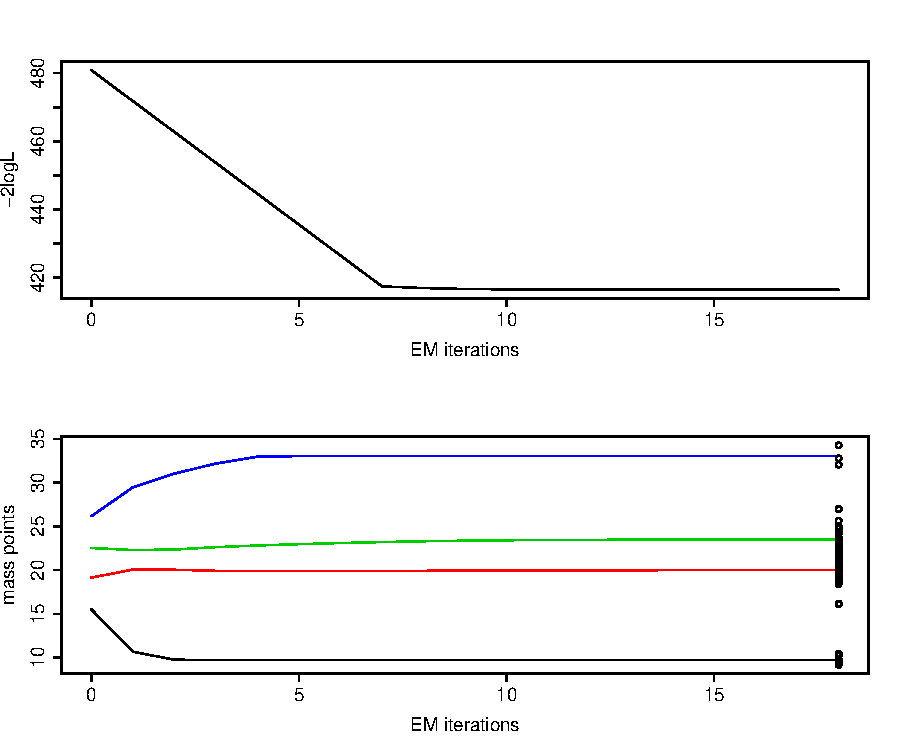
\includegraphics{npmlreg-v-008}

Fig. 1: Convergence of EM algorithm for NPML estimation with 4 mass points.  Top: Disparities; Bottom: EM Trajectories.
\end{minipage}

As {\tt random.distribution='np'} is the default setting, it can  be omitted. For 5 to 9 mass points, we only report the disparity values
%9
\begin{Schunk}
\begin{Sinput}
> (galaxy.np5 <- alldist(v1000 ~ 1, random = ~1, k = 5, data = gal, 
+     verbose = FALSE))$disp
\end{Sinput}
\begin{Soutput}
[1] 410.6852
\end{Soutput}
\begin{Sinput}
> (galaxy.np6 <- alldist(v1000 ~ 1, random = ~1, k = 6, tol = 0.2, 
+     data = gal, verbose = FALSE))$disp
\end{Sinput}
\begin{Soutput}
[1] 394.5811
\end{Soutput}
\begin{Sinput}
> (galaxy.np7 <- alldist(v1000 ~ 1, random = ~1, k = 7, tol = 0.12, 
+     data = gal, verbose = FALSE))$disp
\end{Sinput}
\begin{Soutput}
[1] 388.8639
\end{Soutput}
\begin{Sinput}
> (galaxy.np8 <- alldist(v1000 ~ 1, random = ~1, k = 8, tol = 0.2, 
+     data = gal, verbose = FALSE))$disp
\end{Sinput}
\begin{Soutput}
[1] 388.177
\end{Soutput}
\begin{Sinput}
> (galaxy.np9 <- alldist(v1000 ~ 1, random = ~1, k = 9, tol = 0.06, 
+     data = gal, verbose = FALSE))$disp
\end{Sinput}
\begin{Soutput}
[1] 388.2149
\end{Soutput}
\end{Schunk}
indicating that the disparity stabilizes at about 8 mass points. Note that in some cases it was necessary to modify the optional parameter {\tt tol} 
to obtain the disparity values given above. The {\tt tol} parameter influences the position of the starting points, where
values {\tt tol} $< 1$ mean concentrated values compared to the default setting (Gaussian quadrature points).  The disparity values
for 2 and 5 mass points are better than those obtained by Aitkin (2001) with GLIM 4.  
One reason for that is the applied damping procedure: As the algorithm is less sensitive to the optimal choice of {\tt tol}, 
the optimal solutions are found more easily.  An assisting tool in the selection of {\tt tol} is the R function {\tt tolfind} included in  
the package {\bf npmlreg}. 


To fit a Gaussian mixture with unequal standard deviations $\sigma_k$, $k=1, \ldots, K$ varying over the components, the possibility of smoothing the standard 
deviations among components is implemented. Smoothing is performed by means of the discrete kernel
\[
W(x,y|\lambda)=\left\{\begin{array}{lcc}\lambda &\mbox{if}  & y=x\\
                                        (1-\lambda)/(K-1)   &\mbox{if}  &y \not= x\\
                       \end{array}\right.
                        \]
(Aitchison and Aitken, 1976). The setting $\lambda=1/K$  corresponds to the extreme case `maximal smoothing' (i.e. equal 
variances $\sigma^2=\sigma^2_k$.), while $\lambda = 1$ means that all standard deviations are calculated within the
    components (i.e. unequal variances $\sigma^2_k$).   Statistically sensible settings are only
    $1/K \le  \lambda  \le 1$.  The default setting $\lambda= 0$ is automatically mapped to 
$\lambda =1/K$.  

 As an example, we compute the four  mass-points model with option {\tt lambda=1}
%10
\begin{Schunk}
\begin{Sinput}
> summary(galaxy.np4u <- alldist(v1000 ~ 1, random = ~1, k = 4, 
+     tol = 0.5, data = gal, lambda = 1, verbose = FALSE))
\end{Sinput}
\begin{Soutput}
Call:  alldist(formula = v1000 ~ 1, random = ~1, data = gal, k = 4,      tol = 0.5, lambda = 1, verbose = FALSE) 

Coefficients:
       Estimate Std. Error   t value
MASS1  9.710143  0.2776679  34.97035
MASS2 19.949549  0.1174379 169.87311
MASS3 23.135282  0.1281410 180.54545
MASS4 33.044336  0.4241453  77.90805

Mixture proportions:
     MASS1       MASS2       MASS3       MASS4  
0.08536585  0.47707433  0.40097456  0.03658525  

MLE of component standard deviations:
    MASS1      MASS2      MASS3      MASS4  
0.4225107  1.3831150  1.6866727  0.9217176  

Random effect distribution - standard deviation:	   4.302845 

-2 log L:	    405     Convergence at iteration  31
\end{Soutput}
\end{Schunk}

One gets deeper insight into the fitted model looking at diagnostic plots. Calling

%11
\begin{Schunk}
\begin{Sinput}
> plot(galaxy.np4u, plot.opt = 15, height = 5)
\end{Sinput}
\end{Schunk}

\noindent gives the disparities and EM trajectories as above (Fig. 2 top), and additionally two plots showing the empirical Bayes predictions
vs the true responses, and the component posterior probabilities ($w_{ik}$) against the fixed part residuals ($y_i-x_i\hat{\beta}$), respectively. In the former plot (Fig. 2 left bottom), one sees nicely how  the
predicted values are `flattened' within the custers and smoothed between. In the latter plot (Fig. 2 right bottom), one gets an impression 
of the discriminatory power of the mixture components. Throughout all plots, one colour corresponds to the same particular mass point.

An important remark should be given here: Interpretation (and definition!) of the deviance $D=-2\phi\log L + 2\phi\log L_{saturated}$, provided in {\tt \$deviance}, is not clear when using unequal 
dispersion parameters. In the present implementation, deviances are calculated in this case in a somewhat makeshift manner using the {\it equal} dispersion parameter for the $\phi$ preceding the log-likelihood, and the {\it unequal} dispersion parameters within the log-likelihood.
Hence, it is strictly recommended to work with the disparity rather with the deviance in the case of unequal component dispersion parameters, as the the disparity does not share this problem. This is also
the reason why we prefer to work with disparities in general, and why disparities (and not deviances) are displayed in the summaries.  

%12
\begin{minipage}{21cm}
%\includegraphics[height=13cm,width=15cm]{4uforweb.ps}
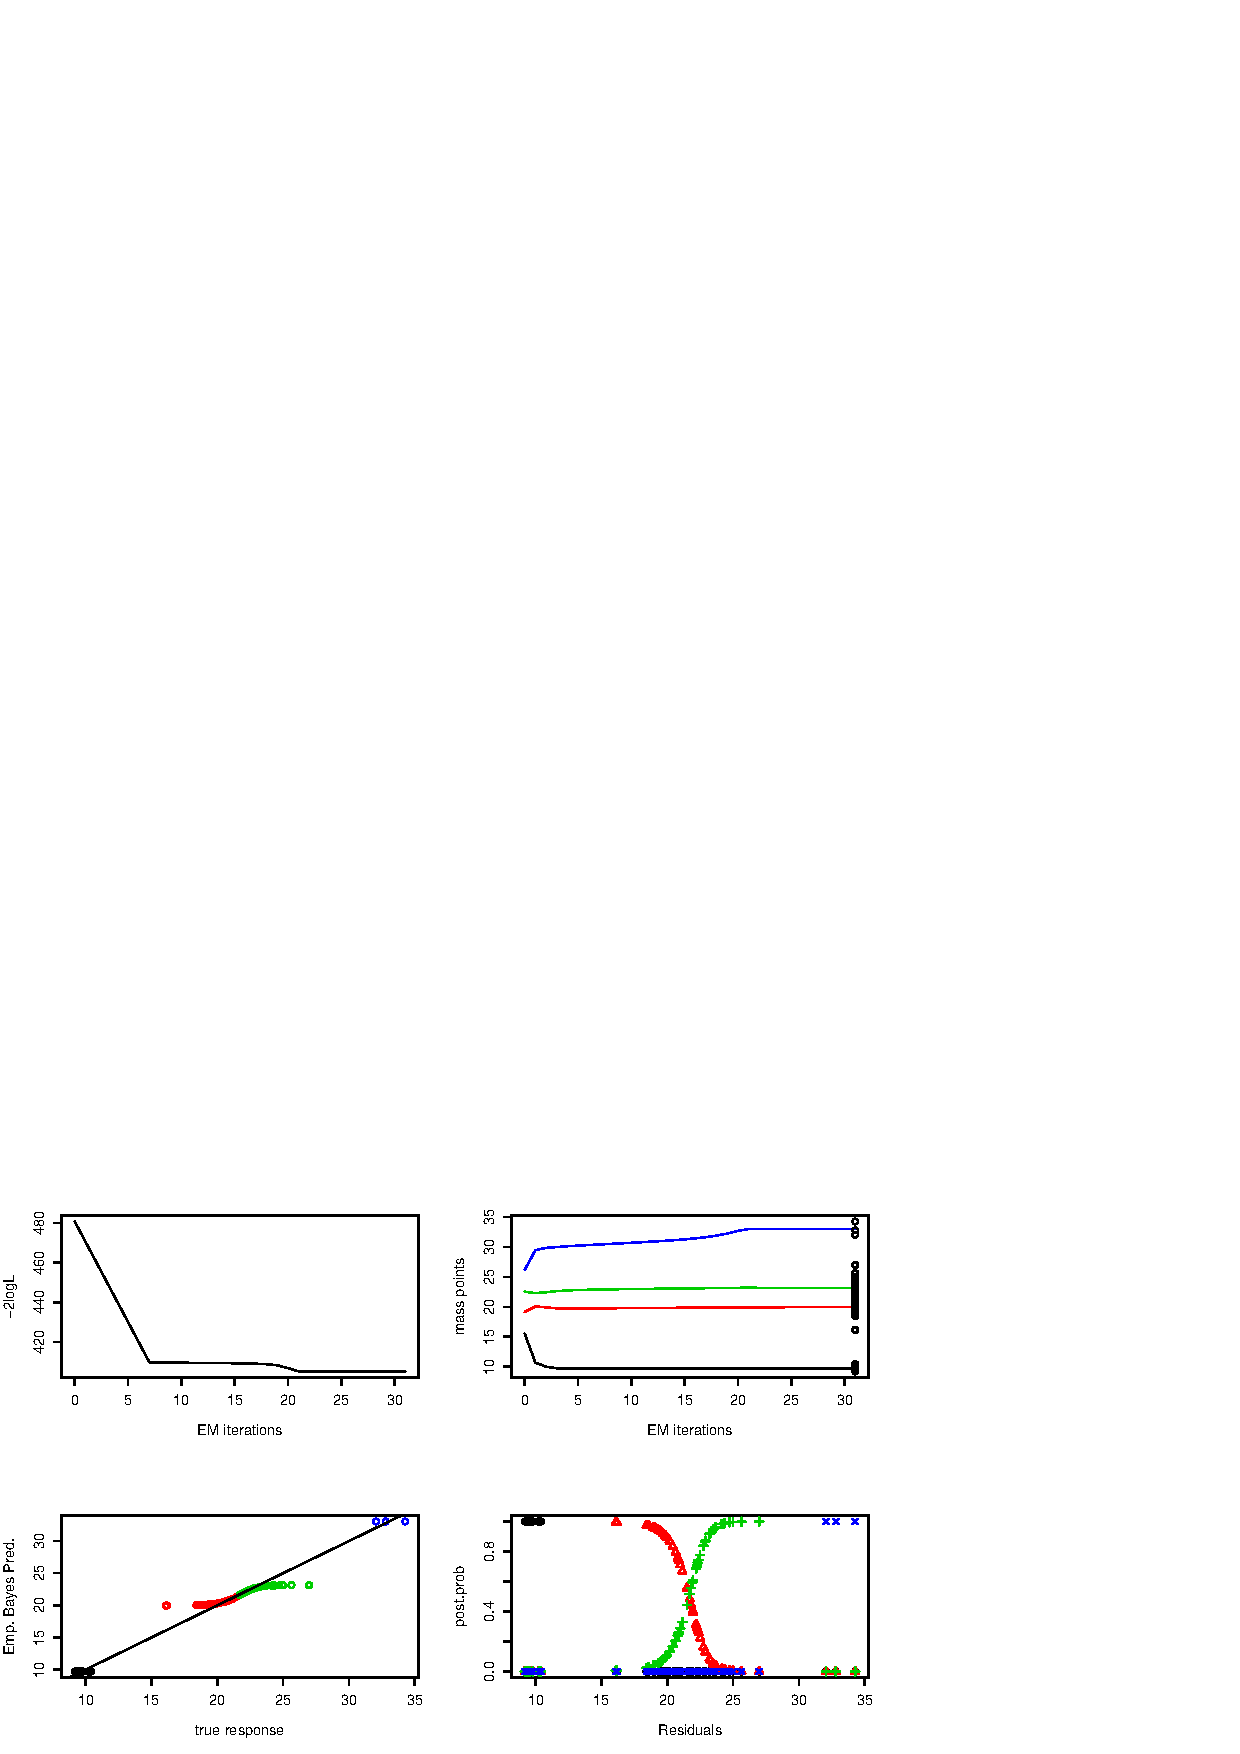
\includegraphics{npmlreg-v-012}

Fig. 2:  Diagnostic plots for NPML estimation with unequal variances and 4 mass points.  
\end{minipage}


One might fear that for a high number of mass points some component  standard deviations could tend to zero. 
This can indeed be the case.  Using  8 instead of 4  mass points in the call above one gets the error message


\vspace{0.3cm}
{\tt 
\noindent  Error in alldist(v1000 ~ 1, random = ~1, k = 8, tol = 0.5, data = gal,  :\\
\indent    Singularity or Likelihood-Spike at iteration \#12.  \\
\indent\indent     Check model specification,  enable spike protection or smooth among components.  \\
}



%Here {\tt \$sdev} gives the 'overall' standard deviation (calculated over all components given the fitted model), and {\tt \$sdevk} the component specific standard deviation. 
%Attention: The 8th mass point is associated with variance zero, resulting in the useless disparity value -373.2.  Such 'likelihood spikes' (Aitkin, Hinde \& Francis, 2005, p. 428) 
%can produce  arbitrarily high likelihoods and consequently arbitrarlily small disparities, 
%which are certainly not at all meaningful. 

This problem may be solved,  as a first attempt, by modifying {\tt tol}. In this case, {\tt tol=0.32} 
gives a likelihood-spike free solution with disparity  357.8, which is a good part better then the value given in Aitkin (2001), 361.0. 
If likelihood spikes occur for any {\tt tol}, one can enable the spike protection ({\tt spike.protect=1}), which stops the algorithm as soon
as one component starts to enter a likelihood spike.  For instance, running

%13
\begin{Schunk}
\begin{Sinput}
> (galaxy.np8us <- alldist(v1000 ~ 1, random = ~1, k = 8, tol = 0.5, 
+     data = gal, lambda = 1, verbose = FALSE, spike.protect = TRUE))
\end{Sinput}
\begin{Soutput}
Call:  alldist(formula = v1000 ~ 1, random = ~1, data = gal, k = 8,      tol = 0.5, lambda = 1, spike.protect = TRUE, verbose = FALSE) 

Coefficients:
 MASS1   MASS2   MASS3   MASS4   MASS5   MASS6   MASS7   MASS8  
 9.383   9.906  17.233  19.772  22.587  24.410  32.433  34.279  

Random effect distribution - standard deviation:	   4.417512 

Mixture proportions:
     MASS1       MASS2       MASS3       MASS4       MASS5       MASS6  
0.03457724  0.05078828  0.03637014  0.37478549  0.35365507  0.11323979  
     MASS7       MASS8  
0.02438886  0.01219512  
-2 log L:	    324.3 
\end{Soutput}
\begin{Sinput}
> galaxy.np8us$sdev$sdevk
\end{Sinput}
\begin{Soutput}
[1] 1.504988e-01 4.113445e-01 1.526060e+00 6.309877e-01 1.170915e+00
[6] 1.738375e+00 3.757823e-01 7.105427e-15
\end{Soutput}
\end{Schunk}

\noindent gives us  estimates of mass points, masses, and standard deviations of the mixture components. These values 
have to be interpreted with care, as the displayed disparity is normally not correct when the algorithm does not have converged. 
One notices from this output that the 8th mass point is responsible for the likelihood spike.

The better approach is to set the smoothing parameter equal to $\lambda=0.99$, 
which corresponds to unequal standard deviations with a very low amount
of smoothing among components:
%14
\begin{Schunk}
\begin{Sinput}
> (galaxy.np8ud <- alldist(v1000 ~ 1, random = ~1, k = 8, tol = 0.5, 
+     data = gal, lambda = 0.99))
\end{Sinput}
\begin{Soutput}
1 ..2 ..3 ..4 ..5 ..6 ..7 ..8 ..9 ..10 ..11 ..12 ..13 ..14 ..15 ..16 ..17 ..18 ..19 ..20 ..21 ..22 ..23 ..24 ..25 ..26 ..27 ..28 ..29 ..30 ..31 ..32 ..33 ..34 ..35 ..36 ..37 ..38 ..39 ..40 ..41 ..42 ..43 ..44 ..45 ..46 ..47 ..48 ..49 ..50 ..51 ..52 ..53 ..54 ..55 ..56 ..57 ..58 ..59 ..60 ..61 ..62 ..63 ..64 ..65 ..66 ..67 ..68 ..69 ..70 ..71 ..72 ..73 ..74 ..75 ..76 ..77 ..78 ..79 ..80 ..81 ..82 ..83 ..84 ..85 ..86 ..87 ..88 ..89 ..90 ..91 ..92 ..93 ..94 ..95 ..96 ..97 ..98 ..99 ..100 ..101 ..102 ..
EM algorithm met convergence criteria at iteration #  102 
Disparity trend plotted.
EM Trajectories plotted.

Call:  alldist(formula = v1000 ~ 1, random = ~1, data = gal, k = 8,      tol = 0.5, lambda = 0.99) 

Coefficients:
 MASS1   MASS2   MASS3   MASS4   MASS5   MASS6   MASS7   MASS8  
 9.836   9.710  16.127  19.790  22.922  26.978  32.427  34.279  

Random effect distribution - standard deviation:	   4.448856 

Mixture proportions:
       MASS1         MASS2         MASS3         MASS4         MASS5  
7.888540e-15  8.536585e-02  2.439018e-02  4.039238e-01  4.256102e-01  
       MASS6         MASS7         MASS8  
2.412464e-02  2.439092e-02  1.219444e-02  
-2 log L:	    374.6 
\end{Soutput}
\begin{Sinput}
> galaxy.np8ud$sdev$sdevk
\end{Sinput}
\begin{Soutput}
[1] 0.9061662 0.4349857 0.2183475 0.6758124 1.2048199 0.2160915 0.4119882
[8] 0.2949645
\end{Soutput}
\end{Schunk}
The motivation for the implementation of {\tt spike.protect} is mainly to enable to run {\tt tolfind}
without breaking down if likelihood spikes occur. Hence, it is in {\tt alldist} by default switched off, 
and in {\tt tolfind} by default switched on.  The result of {\tt tolfind} for the 8-mass point model with unequal variances 
is shown in Fig. 2: Red circles correspond to {\tt tol} values where the spike protection had to interfere and
 hence the EM algorithm did not converge. Only disparity values associated with green circles are reliable, 
 and the  optimal value of {\tt tol} should consequently be chosen from them.
 
 %15
 \begin{minipage}{21cm}
\begin{Schunk}
\begin{Sinput}
> par(mfrow = c(1, 1), cex = 0.65)
> tolfind(v1000 ~ 1, random = ~1, k = 8, data = gal, lambda = 1, 
+     find.in.range = c(0, 0.6), steps = 12, plot.opt = 0, verbose = FALSE, 
+     noformat = TRUE)[c(3, 4)]
\end{Sinput}
\begin{Soutput}
Minimal Disparity: 323.3126 at tol= 0.45 
Minimal Disparity with EM converged: 357.8216 at tol= 0.4 
$AllDisparities
 [1] 1233.6883  387.2360  377.6917  377.0345  360.9393  359.4521  357.8221
 [8]  357.8216  323.3126  324.2868  363.8772       Inf

$Alltol
 [1] 0.05 0.10 0.15 0.20 0.25 0.30 0.35 0.40 0.45 0.50 0.55 0.60
\end{Soutput}
\end{Schunk}
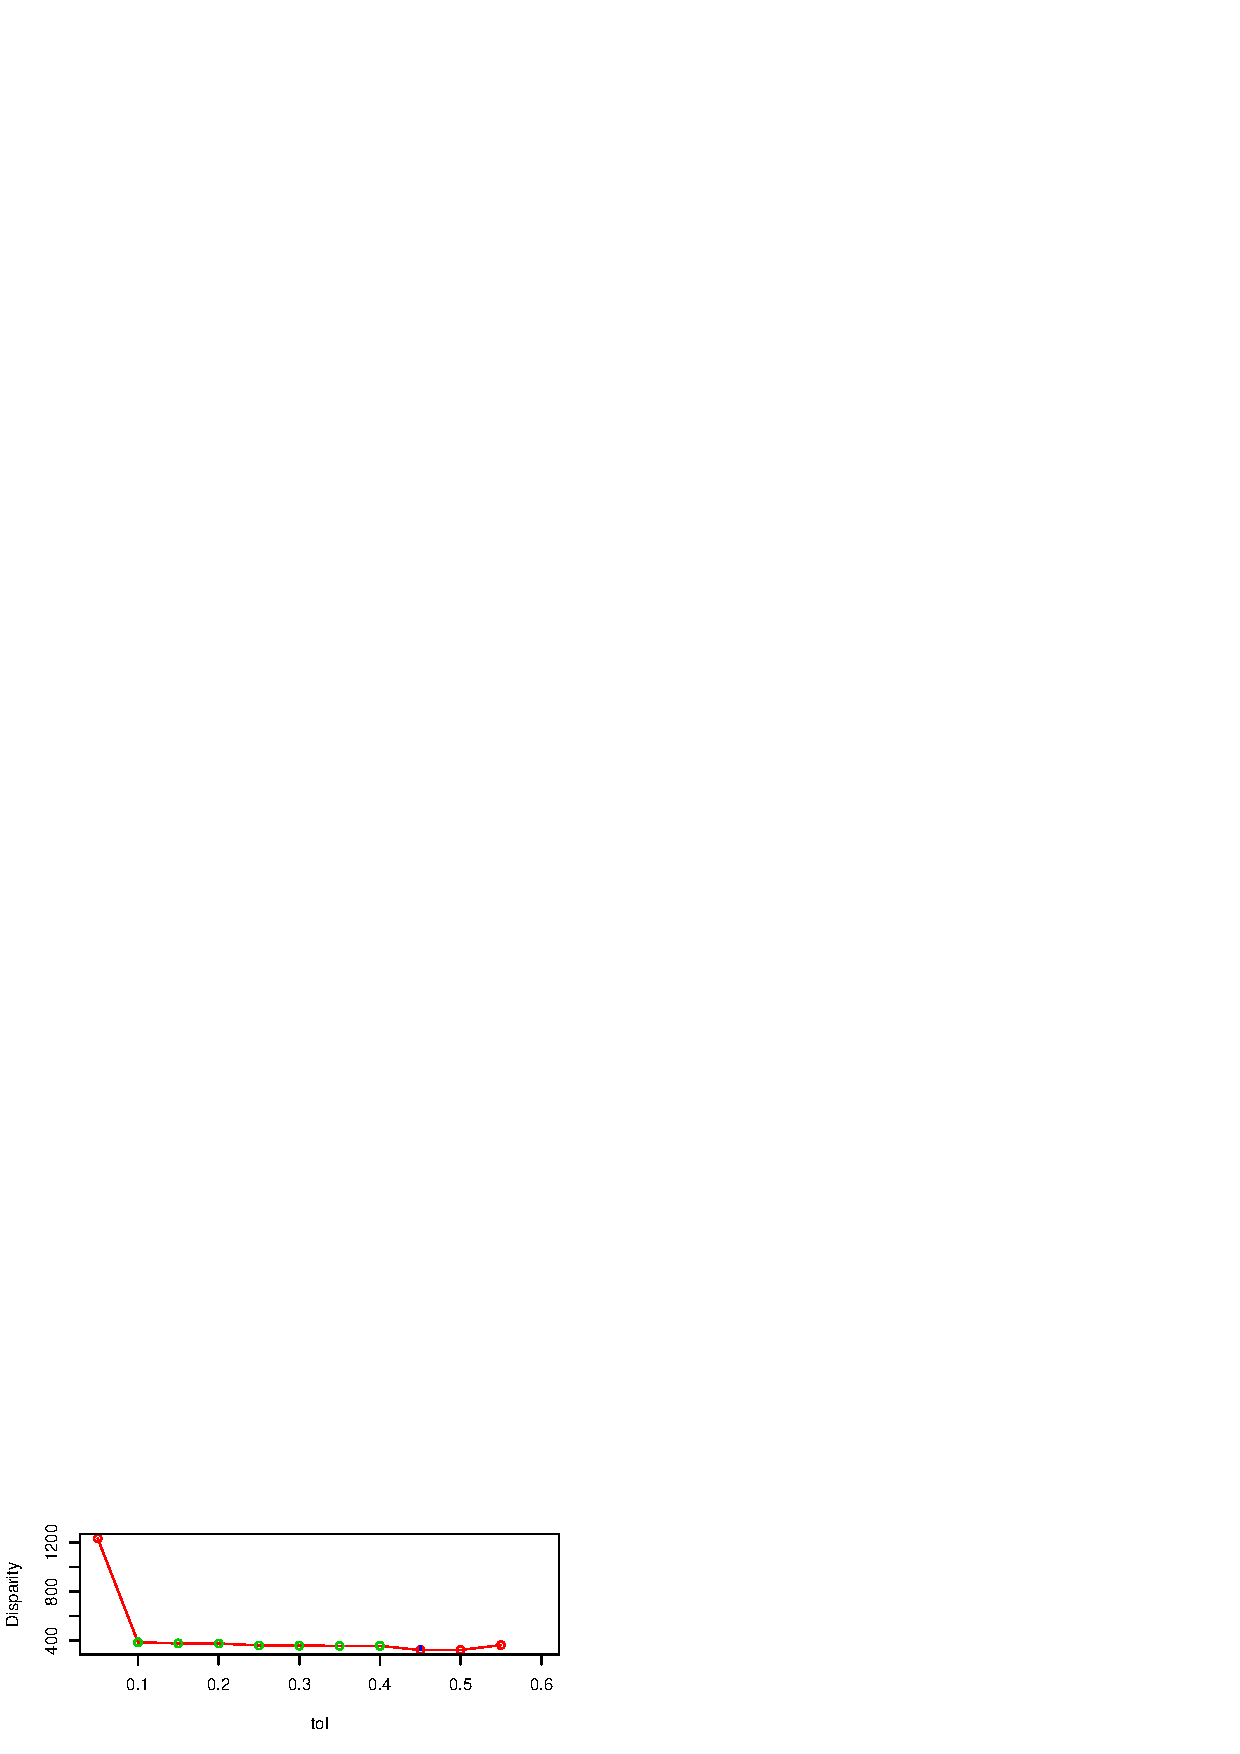
\includegraphics{npmlreg-v-015}
%\includegraphics[height=6cm,width=11cm]{tolfindgal.eps}

Fig. 3: Disparity against {\tt tol} for 8 mass point model with unequal variances. Green circles: EM converged; red circles: EM not converged.
\end{minipage}
 
\subsection{Compound Poisson models: The fabric faults data}

In this Section we consider the fabric faults data,  previously analyzed in Hinde (1982) and  Aitkin,  Francis \& Hinde (2005, p. 453ff). 
This data describes the number of faults in rolls of fabrics with a single covariate {\tt leng} for the length of the roll. The log-length is directly given by the variable {\tt x}.  
The number of faults {\tt y}  can be assumed to follow a Poisson distribution. First, we fit a generalized linear Poisson model with the natural log link
%15
\begin{Schunk}
\begin{Sinput}
> data(fabric, package = "gamlss")
> (faults0 <- glm(y ~ 1, family = poisson(link = log), data = fabric))
\end{Sinput}
\begin{Soutput}
Call:  glm(formula = y ~ 1, family = poisson(link = log), data = fabric) 

Coefficients:
(Intercept)  
      2.183  

Degrees of Freedom: 31 Total (i.e. Null);  31 Residual
Null Deviance:	    103.7 
Residual Deviance: 103.7 	AIC: 229 
\end{Soutput}
\begin{Sinput}
> (faults1 <- glm(y ~ x, family = poisson(link = log), data = fabric))
\end{Sinput}
\begin{Soutput}
Call:  glm(formula = y ~ x, family = poisson(link = log), data = fabric) 

Coefficients:
(Intercept)            x  
     -4.173        0.997  

Degrees of Freedom: 31 Total (i.e. Null);  30 Residual
Null Deviance:	    103.7 
Residual Deviance: 64.54 	AIC: 191.8 
\end{Soutput}
\end{Schunk}
and observe a large reduction in deviance by including the log length.
Fits of count data with Poisson models are often quite poor, as the basic assumption 
underlying a Poisson model, equality of mean and
variance, is often not adequate. 
As a solution, Hinde (1982) proposed to model the unexplained variation by means of a Gaussian random effect $Z$. In case of the fabric fault data,  
one assumes that the number of faults conditional on the observation and on the
random effect follows a Poisson distribution, i.e.
\[
Y|X_1, \ldots, X_n,Z \sim Po(\mu),
\]
where $Z\sim N(0,1)$, and
\[
log(\mu)=c+ log(leng)+\sigma Z,
\]  
 Integrating out the random effect as in (\ref{marginal}), one obtains a Poisson/normal compound distribution, which can
be approximated with Gaussian quadrature (GQ).  For one, two and three mass points one obtains with the log length as covariate: 
%16
\begin{Schunk}
\begin{Sinput}
> (faults.g1 <- alldist(y ~ x, family = poisson(link = log), random = ~1, 
+     data = fabric, k = 1, random.distribution = "gq"))
\end{Sinput}
\begin{Soutput}
Call:  alldist(formula = y ~ x, random = ~1, family = poisson(link = log),      data = fabric, k = 1, random.distribution = "gq") 

Coefficients:
(Intercept)            x  
     -4.173        0.997  
Random effect distribution - standard deviation:	   0 

-2 log L:	    187.8 
\end{Soutput}
\begin{Sinput}
> (faults.g2 <- alldist(y ~ x, family = poisson(link = log), random = ~1, 
+     data = fabric, k = 2, random.distribution = "gq"))
\end{Sinput}
\begin{Soutput}
1 ..2 ..3 ..4 ..5 ..6 ..
EM algorithm met convergence criteria at iteration #  6 
Disparity trend plotted.

Call:  alldist(formula = y ~ x, random = ~1, family = poisson(link = log),      data = fabric, k = 2, random.distribution = "gq") 

Coefficients:
(Intercept)            x            z  
    -4.4128       1.0331       0.3391  
Random effect distribution - standard deviation:	   0.3391081 

-2 log L:	    175.6 
\end{Soutput}
\begin{Sinput}
> (faults.g3 <- alldist(y ~ x, family = poisson(link = log), random = ~1, 
+     data = fabric, k = 3, random.distribution = "gq", verbose = F))
\end{Sinput}
\begin{Soutput}
Call:  alldist(formula = y ~ x, random = ~1, family = poisson(link = log),      data = fabric, k = 3, random.distribution = "gq", verbose = F) 

Coefficients:
(Intercept)            x            z  
    -3.3089       0.8488       0.3575  
Random effect distribution - standard deviation:	   0.3574909 

-2 log L:	    174.3 
\end{Soutput}
\end{Schunk}
The one mass point model is equivalent to the model {\tt faults1} given above, which can also be verified by checking the deviance
%17
\begin{Schunk}
\begin{Sinput}
> faults.g1$dev
\end{Sinput}
\begin{Soutput}
[1] 64.53719
\end{Soutput}
\end{Schunk}
For a Poisson model, deviance and disparity are related by the equation
$D=Disp +2L_{sat}$
and are consequently equal up to an additive constant (the double saturated likelihood), which in our case takes  the value $123.30$. Thus, the disparity 
 174.3 for three mass points corresponds exactly to the deviance value of 51.0 reported in Hinde (1982), p. 119. For comparison, one can also fit the two and three mass point models
 with NPML:
 %18
\begin{Schunk}
\begin{Sinput}
> (faults.np2 <- alldist(y ~ x, family = poisson(link = log), random = ~1, 
+     data = fabric, k = 2, random.distribution = "np"))
\end{Sinput}
\begin{Soutput}
1 ..2 ..3 ..4 ..5 ..6 ..7 ..8 ..9 ..10 ..11 ..12 ..13 ..14 ..15 ..16 ..17 ..18 ..19 ..20 ..21 ..22 ..
EM algorithm met convergence criteria at iteration #  22 
Disparity trend plotted.
EM Trajectories plotted.

Call:  alldist(formula = y ~ x, random = ~1, family = poisson(link = log),      data = fabric, k = 2, random.distribution = "np") 

Coefficients:
      x    MASS1    MASS2  
 0.8045  -3.1645  -2.4017  

Random effect distribution - standard deviation:	   0.3084855 

Mixture proportions:
    MASS1      MASS2  
0.7940023  0.2059977  
-2 log L:	    172.7 
\end{Soutput}
\begin{Sinput}
> (faults.np3 <- alldist(y ~ x, family = poisson(link = log), random = ~1, 
+     data = fabric, k = 3, random.distribution = "np", verbose = FALSE))
\end{Sinput}
\begin{Soutput}
Call:  alldist(formula = y ~ x, random = ~1, family = poisson(link = log),      data = fabric, k = 3, random.distribution = "np", verbose = FALSE) 

Coefficients:
     x   MASS1   MASS2   MASS3  
 0.798  -3.154  -3.114  -2.353  

Random effect distribution - standard deviation:	   0.307822 

Mixture proportions:
    MASS1      MASS2      MASS3  
0.1319235  0.6666708  0.2014057  
-2 log L:	    172.7 
\end{Soutput}
\end{Schunk}
The disparities are not far from those obtained with Gaussian quadrature, indicating that the random effect distribution is 
not very far from a normal distribution.  While three mass points seem to be adequate for GQ, only two mass points are needed with NPML.
Note that the use of option {\tt random.distribution="np"} yields an object of type {\tt glmmNPML}, while  option {\tt random.distribution="gq"} yields an object of type {\tt glmmGQ}.
 
 Predictions  for objects of type {\tt glmmGQ} can
 be obtained  by 
%19
\begin{Schunk}
\begin{Sinput}
> predict(faults.g2, type = "response", newdata = fabric[1:6, ])
\end{Sinput}
\begin{Soutput}
      1       2       3       4       5       6 
 8.7158 10.3546 13.3412  5.8568 11.4078 13.9380 
\end{Soutput}
\end{Schunk}
or
%20
\begin{Schunk}
\begin{Sinput}
> predict(faults.g2, type = "response")[1:6]
\end{Sinput}
\begin{Soutput}
      1       2       3       4       5       6 
 6.5578  7.0462 17.0202  7.2890 13.9926  9.5338 
\end{Soutput}
\end{Schunk}
which both call function {\tt predict.glmmGQ}. The results of the two predictions differ, 
since in the first case prediction is done using the analytical mean of the marginal distribution, considering {\tt faults[1:6,]} as `new' input data (Aitkin, Hinde \& Francis,  2005, p. 459),  
and in the second case in an  empirical Bayes approach (Aitkin, 1996a) using the individual posterior probabilities 
obtained as a by-product of the EM algorithm.  
 
 
  
\subsection{Logistic regression with random effects: The toxoplasmosis data} 
 
The toxoplasmosis data, also called rainfall data, are available via 
%21
\begin{Schunk}
\begin{Sinput}
> data(rainfall, package = "forward")
> rainfall$x <- rainfall$Rain/1000
> rainfall$x2 <- rainfall$x^2
> rainfall$x3 <- rainfall$x^3
\end{Sinput}
\end{Schunk}
gives the number of subjects {\tt Cases} out of {\tt Total} testing positively for toxoplasmosis
in each of 34 cities in El Salvador with annual rainfall  {\tt x} in 1000 mm. The data have been 
 analyzed in Efron (1998) using generalized linear models and   in Aitkin \& Francis (1995) using the GLIM 4 implementation of
 NPML. Fitting, as the latter authors, a constant logistic overdispersion model with three mass points, one obtains
  %22
\begin{Schunk}
\begin{Sinput}
> (toxo.np <- alldist(cbind(Cases, Total - Cases) ~ 1, random = ~1, 
+     data = rainfall, k = 3, family = binomial(link = logit)))
\end{Sinput}
\begin{Soutput}
1 ..2 ..3 ..4 ..5 ..6 ..7 ..8 ..9 ..10 ..11 ..12 ..
EM algorithm met convergence criteria at iteration #  12 
Disparity trend plotted.
EM Trajectories plotted.

Call:  alldist(formula = cbind(Cases, Total - Cases) ~ 1, random = ~1,      family = binomial(link = logit), data = rainfall, k = 3) 

Coefficients:
  MASS1    MASS2    MASS3  
-0.9793   0.1492   0.7615  

Random effect distribution - standard deviation:	   0.5996584 

Mixture proportions:
     MASS1       MASS2       MASS3  
0.33421659  0.57062599  0.09515743  
-2 log L:	    146.9 
\end{Soutput}
\end{Schunk}
 The result is approximately the same as that obtained by Aitkin \& Francis (1995). However, note that the disparity
   %23
\begin{Schunk}
\begin{Sinput}
> toxo.np$disparity
\end{Sinput}
\begin{Soutput}
[1] 146.8668
\end{Soutput}
\end{Schunk}
 differs from the GLIM 4 result $947.89$. The disparity for binomial models provided by GLIM 4 has to be interpreted as  $-2\log L+c$, where $c$ is some 
 additive constant only depending on the values of {\tt y } and {\tt n}, while the disparity given by this R implementation 
 is just $-2\log L$. 
 Adding rainfall as fixed effect, we fit a linear random effect model
 %24
\begin{Schunk}
\begin{Sinput}
> (toxo.npx <- alldist(cbind(Cases, Total - Cases) ~ x, random = ~1, 
+     data = rainfall, k = 3, family = binomial(link = logit)))
\end{Sinput}
\begin{Soutput}
1 ..2 ..3 ..4 ..5 ..6 ..7 ..8 ..9 ..10 ..11 ..12 ..
EM algorithm met convergence criteria at iteration #  12 
Disparity trend plotted.
EM Trajectories plotted.

Call:  alldist(formula = cbind(Cases, Total - Cases) ~ x, random = ~1,      family = binomial(link = logit), data = rainfall, k = 3) 

Coefficients:
      x    MASS1    MASS2    MASS3  
 0.2897  -1.5494  -0.4063   0.2385  

Random effect distribution - standard deviation:	   0.6059427 

Mixture proportions:
    MASS1      MASS2      MASS3  
0.3321544  0.5787877  0.0890579  
-2 log L:	    146.6 
\end{Soutput}
\end{Schunk}
   The decrease in disparity compared to the constant model is only 0.3 on 1df (and is 5.1 for a cubic model, on 3df). %for the linear model and 5.03 on 3df for the cubic model.
 We also try a random slope
 %25
\begin{Schunk}
\begin{Sinput}
> (toxo.npxx <- alldist(cbind(Cases, Total - Cases) ~ x, random = ~x, 
+     data = rainfall, k = 3, family = binomial(link = logit)))
\end{Sinput}
\begin{Soutput}
1 ..2 ..3 ..4 ..5 ..6 ..7 ..8 ..9 ..10 ..11 ..12 ..
EM algorithm met convergence criteria at iteration #  12 
Disparity trend plotted.
EM Trajectories plotted.

Call:  alldist(formula = cbind(Cases, Total - Cases) ~ x, random = ~x,      family = binomial(link = logit), data = rainfall, k = 3) 

Coefficients:
      x    MASS1    MASS2    MASS3  MASS1:x  MASS2:x  
-0.6688  -0.2451  -0.7948   2.0048   0.3038   1.1590  

Random effect distribution - standard deviation:	   0.8089833 

Mixture proportions:
     MASS1       MASS2       MASS3  
0.33569914  0.56715671  0.09714415  
-2 log L:	    146.1 
\end{Soutput}
\end{Schunk}
 giving only a negligible decrease in disparity compared to the linear fixed effects model.  All in all, when accounting for overdispersion, 
 there is no  overwhelming evidence that rainfall has a significant influence on the incidence of toxoplasmosis at all.
 
 For the simple constant model, the posteriori probabilities $w_{ik}$
  %26
\begin{Schunk}
\begin{Sinput}
> round(t(toxo.np$post.prob), digits = 2)
\end{Sinput}
\begin{Soutput}
     1    2    3    4    5    6    7    8    9   10   11   12   13   14   15
1 0.25 0.64 0.63 0.64 0.11 0.14 0.69 0.53 0.21 0.00 0.92 0.45 0.02 0.99 0.45
2 0.67 0.35 0.35 0.35 0.70 0.74 0.30 0.46 0.71 0.65 0.08 0.49 0.96 0.01 0.49
3 0.09 0.01 0.02 0.01 0.19 0.12 0.01 0.00 0.08 0.35 0.00 0.06 0.02 0.00 0.06
    16   17   18   19   20   21   22   23 24   25   26   27   28   29   30   31
1 0.08 0.45 0.00 0.26 0.87 0.93 0.45 0.01  0 0.01 0.22 0.00 0.01 0.00 0.00 0.02
2 0.83 0.49 0.86 0.69 0.12 0.07 0.49 0.73  1 0.99 0.75 0.99 0.75 0.98 0.07 0.83
3 0.09 0.06 0.14 0.05 0.00 0.00 0.06 0.27  0 0.00 0.02 0.01 0.24 0.02 0.93 0.14
    32   33   34
1 0.64 0.73 0.00
2 0.35 0.26 0.82
3 0.01 0.01 0.18
\end{Soutput}
\end{Schunk}
 show how the observations are allocated to the mass points, indicating that actually only one observation (the 30th) 
 represents the 3rd mass point. From the posteriori probabilites, one also obtains the empirical
 Bayes predictions
 $
\tilde{\eta}_i=\sum_k \hat{\eta}_{ik}\hat{w}_{ik}
 $
  as in Aitkin (1996b),  from which the predicted toxoplasmosis incidence probabilities $\tilde{p}_i=\exp(\tilde{\eta}_i)/(1+\exp(\tilde{\eta}_i))$ can be calculated: 
%27
\begin{Schunk}
\begin{Sinput}
> round(toxo.ebp <- toxo.np$ebp, digits = 3)
\end{Sinput}
\begin{Soutput}
     1      2      3      4      5      6      7      8      9     10     11 
-0.079 -0.566 -0.555 -0.566  0.146  0.065 -0.622 -0.450 -0.041  0.356 -0.885 
    12     13     14     15     16     17     18     19     20     21     22 
-0.326  0.140 -0.971 -0.326  0.114 -0.326  0.237 -0.115 -0.838 -0.902 -0.326 
    23     24     25     26     27     28     29     30     31     32     33 
 0.304  0.152  0.139 -0.090  0.157  0.290  0.162  0.719  0.214 -0.566 -0.673 
    34 
 0.257 
\end{Soutput}
\begin{Sinput}
> round(exp(toxo.ebp)/(1 + exp(toxo.ebp)), digits = 4)
\end{Sinput}
\begin{Soutput}
     1      2      3      4      5      6      7      8      9     10     11 
0.4803 0.3622 0.3647 0.3622 0.5363 0.5161 0.3494 0.3893 0.4899 0.5882 0.2921 
    12     13     14     15     16     17     18     19     20     21     22 
0.4193 0.5350 0.2747 0.4193 0.5284 0.4193 0.5590 0.4714 0.3020 0.2886 0.4193 
    23     24     25     26     27     28     29     30     31     32     33 
0.5754 0.5379 0.5347 0.4775 0.5393 0.5720 0.5403 0.6725 0.5534 0.3622 0.3378 
    34 
0.5638 
\end{Soutput}
\end{Schunk}
This can alternatively be done easier by using the generic predict function,
%28
\begin{Schunk}
\begin{Sinput}
> predict(toxo.np, type = "response")
\end{Sinput}
\begin{Soutput}
     1      2      3      4      5      6      7      8      9     10     11 
0.4803 0.3622 0.3647 0.3622 0.5363 0.5161 0.3494 0.3893 0.4899 0.5882 0.2921 
    12     13     14     15     16     17     18     19     20     21     22 
0.4193 0.5350 0.2747 0.4193 0.5284 0.4193 0.5590 0.4714 0.3020 0.2886 0.4193 
    23     24     25     26     27     28     29     30     31     32     33 
0.5754 0.5379 0.5347 0.4775 0.5393 0.5720 0.5403 0.6725 0.5534 0.3622 0.3378 
    34 
0.5638 
\end{Soutput}
\end{Schunk}
or, even quicker,
\begin{Schunk}
\begin{Sinput}
> fitted(toxo.np)
\end{Sinput}
\begin{Soutput}
        1         2         3         4         5         6         7         8 
0.4802916 0.3621653 0.3646799 0.3621653 0.5363293 0.5161203 0.3493630 0.3893228 
        9        10        11        12        13        14        15        16 
0.4898596 0.5881705 0.2920528 0.4193273 0.5350387 0.2747238 0.4193273 0.5283871 
       17        18        19        20        21        22        23        24 
0.4193273 0.5589992 0.4713726 0.3019893 0.2885689 0.4193273 0.5753992 0.5378508 
       25        26        27        28        29        30        31        32 
0.5347178 0.4775425 0.5392603 0.5719516 0.5403452 0.6724540 0.5533823 0.3621653 
       33        34 
0.3377802 0.5637801 
\end{Soutput}
\end{Schunk}
 which call function {\tt predict.glmmNPML} for an object of type {\tt glmmNPML}. 
 The predict function can also be used to obtain predictions for new input values, e.g. for the linear random effect model:
%29
\begin{Schunk}
\begin{Sinput}
> predict(toxo.npx, type = "response", newdata = data.frame(x = 2))
\end{Sinput}
\begin{Soutput}
     1 
0.4628 
\end{Soutput}
\end{Schunk}

\subsection{Modelling mixtures of Gamma distributions: The hospital stay data} 
 
The hospital-stay data is a sample from a larger data set collected on persons
discharged from a Pennsylvania hospital as part of a retrospective
chart review of antibiotic use in
hospitals (Rosner, 2000, p. 39). 
Relevant covariates of the data set 
are {\tt temp1} (the first measured temperature following admission,
measured in Fahrenheit) and {\tt age}, and the response is the duration of hospital stay.
We read the data in and fit a three mass point model  via
%30
\begin{Schunk}
\begin{Sinput}
> data(hosp)
> (fitnp3 <- alldist(duration ~ age + temp1, data = hosp, k = 3, 
+     family = Gamma(link = log), tol = 0.2))
\end{Sinput}
\begin{Soutput}
1 ..2 ..3 ..4 ..5 ..6 ..7 ..8 ..9 ..10 ..11 ..12 ..13 ..14 ..15 ..16 ..17 ..18 ..19 ..20 ..21 ..22 ..23 ..24 ..25 ..26 ..27 ..
EM algorithm met convergence criteria at iteration #  27 
Disparity trend plotted.
EM Trajectories plotted.

Call:  alldist(formula = duration ~ age + temp1, family = Gamma(link = log),      data = hosp, k = 3, tol = 0.2) 

Coefficients:
       age       temp1       MASS1       MASS2       MASS3  
  0.004028    0.357537  -33.801628  -33.021757  -32.369541  

Component distribution - MLE of shape parameter:	   50.78 
Random effect distribution - standard deviation:	   0.5069548 

Mixture proportions:
    MASS1      MASS2      MASS3  
0.4798559  0.3980453  0.1220988  
-2 log L:	    121.3 
\end{Soutput}
\end{Schunk}
giving the estimated shape parameter
 %31
\begin{Schunk}
\begin{Sinput}
> fitnp3$shape
\end{Sinput}
\begin{Soutput}
$shape
[1] 50.78155

$shapek
[1] 50.78155 50.78155 50.78155
\end{Soutput}
\end{Schunk}

(Certainly, all three component shape parameters listet at {\tt \$shapek} are equal, as by default all components are assumed 
to have the same dispersion parameter.) For comparison, a three mass point mixture of exponentials (i.e. shape=1) is significantly inferior, yielding
%32
\begin{Schunk}
\begin{Sinput}
> (fitnp3e <- alldist(duration ~ age + temp1, data = hosp, k = 3, 
+     family = Gamma(link = log), tol = 0.2, shape = 1))
\end{Sinput}
\begin{Soutput}
1 ..2 ..3 ..4 ..5 ..6 ..7 ..8 ..9 ..10 ..11 ..12 ..13 ..14 ..15 ..16 ..17 ..18 ..19 ..20 ..21 ..22 ..23 ..24 ..25 ..26 ..27 ..28 ..29 ..30 ..31 ..32 ..33 ..34 ..35 ..36 ..37 ..38 ..39 ..40 ..41 ..
EM algorithm met convergence criteria at iteration #  41 
Disparity trend plotted.
EM Trajectories plotted.

Call:  alldist(formula = duration ~ age + temp1, family = Gamma(link = log),      data = hosp, k = 3, tol = 0.2, shape = 1) 

Coefficients:
     age     temp1     MASS1     MASS2     MASS3  
  0.0149    0.3066  -28.6541  -28.6541  -28.6541  

Component distribution - MLE of shape parameter:	   1 
Random effect distribution - standard deviation:	   1.753596e-14 

Mixture proportions:
    MASS1      MASS2      MASS3  
0.2295706  0.5465535  0.2238760  
-2 log L:	    155.2 
\end{Soutput}
\end{Schunk}
 
 For a more detailed analysis of this data set see Einbeck \& Hinde (2006).
 
One important remark should still be given. When employing the damped EM algorithm, 
one will very occasionally observe rising disparities, typically from about the 10th to the 30th EM iteration. 
According to the theory on EM, this shouldn't happen. This phenomenon occurs as 
 the damping step modifies the likelihood,  and hence the theoretical basis for EM is not given any more. 
 {\it Damped} EM is actually only {\it asymptotical} EM, 
 as for a large number of iterations the effect of damping vanishes.  It depends on the application
 and on {\tt tol} what is a `large' number of iterations. In general, rising disparities are more likely to be observed for small values of {\tt tol}  than
 for large values of {\tt tol}, and more likely to be observed for Gamma than for Gaussian mixtures.
   Though these rising disparities are not really a problem, as at convergence the number of
 iterations is generally high enough, one might want to avoid them for esthetic reasons. This can be achieved by setting
 the constant {\tt damp.power} in the formula
 \[
 d_j= 1-(1-\mbox{\tt tol})^{\mbox{\tt damp.power*iter}+1}
 \]
 to a value bigger than one, where {\tt iter}$\equiv j$ is the number of iterations and $d_j$ is the multiplicative 
 constant adjusting the dispersion parameter (Einbeck \& Hinde, 2006). Another alternative is certainly to switch off damping
 (option {\tt damp=FALSE)} but then it will not work at all in some cases.
 
 
  
 
 

 

 \subsection{Variance component models: The Oxford school boys data}
 
 This data set, also analyzed in Goldstein (2003), contains the heights of 26 boys in Oxford, measured on
 nine occasions over two years. The data set is contained in the R library {\tt nlme} and can 
 be loaded and plotted via
 
 %33
 \begin{minipage}{21cm}
 %\includegraphics[height=12cm,width=23cm]{boys.ps}
\begin{Schunk}
\begin{Sinput}
> data(Oxboys, package = "nlme")
> Oxboys$boy <- gl(26, 9)
> plot(Oxboys$age[Oxboys$boy == 1], Oxboys$height[Oxboys$boy == 
+     1], ylim = c(125, 175), type = "b", pch = 1, xlab = "age", 
+     ylab = "height")
> for (i in 2:nlevels(Oxboys$Subject)) {
+     lines(Oxboys$age[Oxboys$boy == i], Oxboys$height[Oxboys$boy == 
+         i], pch = 1, type = "b", col = i)
+ }
\end{Sinput}
\end{Schunk}
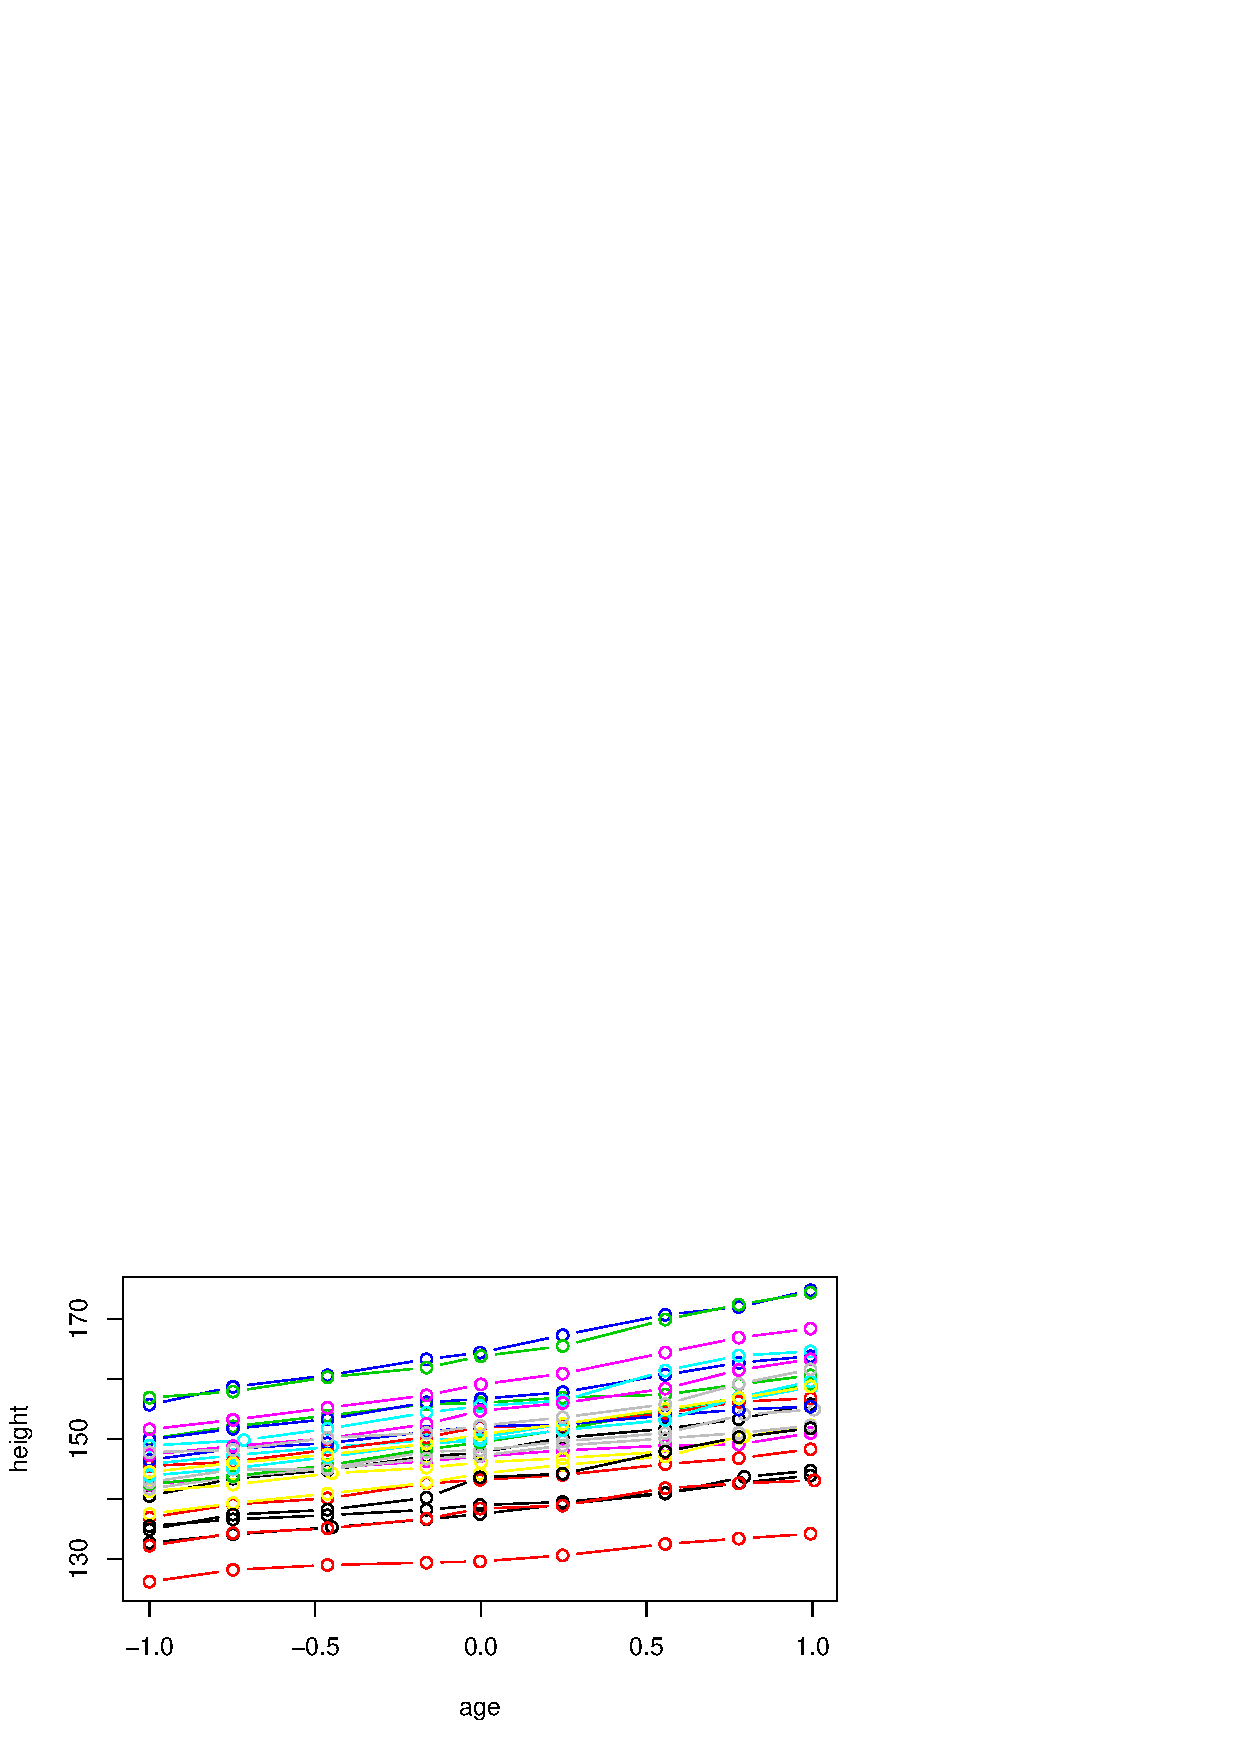
\includegraphics{npmlreg-v-035}
 
 Fig. 4:  Oxford Boys Data %, 
\end{minipage}

 The boys represent the upper level 
 (primary sampling units, PSU), and the particular measurements at different time points 
 correspond to the lower-level units 
 (secondary sampling units, SSU).   Fitting a variance component model with Gaussian quadrature
  (20 mass points), one gets
 %34
\begin{Schunk}
\begin{Sinput}
> (Oxboys.g20 <- allvc(height ~ age, random = ~1 | boy, data = Oxboys, 
+     random.distribution = "gq", k = 20))
\end{Sinput}
\begin{Soutput}
1 ..2 ..3 ..4 ..5 ..6 ..7 ..8 ..9 ..10 ..11 ..12 ..13 ..14 ..15 ..
EM algorithm met convergence criteria at iteration #  15 
Disparity trend plotted.

Call:  allvc(formula = height ~ age, random = ~1 | boy, data = Oxboys,      k = 20, random.distribution = "gq") 

Coefficients:
(Intercept)          age            z  
    148.958        6.524        4.769  

Component distribution - MLE of sigma:	   1.506 
Random effect distribution - standard deviation:	   4.76949 

-2 log L:	    991.8 
\end{Soutput}
\end{Schunk}
This is no satisfactory solution since fitting the same data with function {\tt lmer} in R package {\bf lme4} gives a disparity of 940.6,  as pointed out by Einbeck, Hinde \& Darnell (2007). It turns out that a huge number of mass points $K \approx 500$ is needed in this example to get down to a similar disparity.  We have observed this phenomenon also at other occasions and it seems to occur only if the intra-class correlation (ICC), given by
\[
 ICC= \frac{\sigma_z^2}{\sigma_z^2+\sigma^2}
\]
is quite large. For example, for the model fitted above it is
%35
\begin{Schunk}
\begin{Sinput}
> Oxboys.g20$rsdev^2/(Oxboys.g20$rsdev^2 + Oxboys.g20$sdev$sdev^2)
\end{Sinput}
\begin{Soutput}
[1] 0.9093017
\end{Soutput}
\end{Schunk}
which is a very large value. We have not observed this problem for smaller ICCs, i.e. roughly $ICC \le 0.5$. Fortunately, the problem does not persist for NPML estimation. For illustration, we fit NPML with seven (as suggested by Aitkin, Hinde \& Francis (2005), p. 495), and eight masspoints,  yielding
%35
\begin{Schunk}
\begin{Sinput}
> (Oxboys.np7 <- allvc(height ~ age, random = ~1 | boy, data = Oxboys, 
+     random.distribution = "np", k = 7))
\end{Sinput}
\begin{Soutput}
1 ..2 ..3 ..4 ..5 ..6 ..7 ..8 ..9 ..10 ..
EM algorithm met convergence criteria at iteration #  10 
Disparity trend plotted.
EM Trajectories plotted.

Call:  allvc(formula = height ~ age, random = ~1 | boy, data = Oxboys,      k = 7, random.distribution = "np") 

Coefficients:
    age    MASS1    MASS2    MASS3    MASS4    MASS5    MASS6    MASS7  
  6.524  130.200  138.417  144.605  149.967  155.261  159.521  164.884  

Component distribution - MLE of sigma:	   1.762 
Random effect distribution - standard deviation:	   7.850653 

Mixture proportions:
     MASS1       MASS2       MASS3       MASS4       MASS5       MASS6  
0.03846154  0.11538462  0.19303307  0.34544795  0.19228146  0.03846828  
     MASS7  
0.07692308  
-2 log L:	    1017.3 
\end{Soutput}
\begin{Sinput}
> (Oxboys.np8 <- allvc(height ~ age, random = ~1 | boy, data = Oxboys, 
+     random.distribution = "np", k = 8))
\end{Sinput}
\begin{Soutput}
1 ..2 ..3 ..4 ..5 ..6 ..7 ..8 ..9 ..10 ..
EM algorithm met convergence criteria at iteration #  10 
Disparity trend plotted.
EM Trajectories plotted.

Call:  allvc(formula = height ~ age, random = ~1 | boy, data = Oxboys,      k = 8, random.distribution = "np") 

Coefficients:
    age    MASS1    MASS2    MASS3    MASS4    MASS5    MASS6    MASS7  
  6.524  130.200  138.417  143.382  147.350  151.267  155.789  159.522  
  MASS8  
164.884  

Component distribution - MLE of sigma:	   1.433 
Random effect distribution - standard deviation:	   7.917343 

Mixture proportions:
     MASS1       MASS2       MASS3       MASS4       MASS5       MASS6  
0.03846154  0.11538462  0.11538469  0.19230765  0.26921962  0.15385725  
     MASS7       MASS8  
0.03846155  0.07692308  
-2 log L:	    931.4 
\end{Soutput}
\end{Schunk}
 Thus, NPML with 8 mass points already leads to a better result than GQ with 20 mass points. 
 The EM trajectories, as shown in Fig. 5, can also be
 obtained explicitly by calling
 
 %36
 
\begin{Schunk}
\begin{Sinput}
> plot(Oxboys.np8, plot.opt = 2)
\end{Sinput}
\end{Schunk}
 
  
 We now extend the 8-point model by allowing the linear trend to vary across boys.
%31
\begin{Schunk}
\begin{Sinput}
> (Oxboys.np8s <- allvc(height ~ age, random = ~age | boy, data = Oxboys, 
+     random.distribution = "np", k = 8))
\end{Sinput}
\begin{Soutput}
1 ..2 ..3 ..4 ..5 ..6 ..7 ..8 ..9 ..10 ..
EM algorithm met convergence criteria at iteration #  10 
Disparity trend plotted.
EM Trajectories plotted.

Call:  allvc(formula = height ~ age, random = ~age | boy, data = Oxboys,      k = 8, random.distribution = "np") 

Coefficients:
      age      MASS1      MASS2      MASS3      MASS4      MASS5      MASS6  
   9.2130   130.2616   138.4476   143.3707   147.3756   151.2646   155.7763  
    MASS7      MASS8  MASS1:age  MASS2:age  MASS3:age  MASS4:age  MASS5:age  
 159.4738   164.8242    -5.4901    -4.0056    -2.1543    -3.7833    -2.5653  
MASS6:age  MASS7:age  
  -2.1239    -0.5421  

Component distribution - MLE of sigma:	   1.185 
Random effect distribution - standard deviation:	   7.893352 

Mixture proportions:
     MASS1       MASS2       MASS3       MASS4       MASS5       MASS6  
0.03846154  0.11538462  0.11538462  0.19230769  0.26923047  0.15384645  
     MASS7       MASS8  
0.03846154  0.07692308  
-2 log L:	    842.4 
\end{Soutput}
\end{Schunk}
 The difference in disparities is
 %37
\begin{Schunk}
\begin{Sinput}
> Oxboys.np8$disp - Oxboys.np8s$disp
\end{Sinput}
\begin{Soutput}
[1] 88.93035
\end{Soutput}
\end{Schunk}
 on 7df, showing clear heterogeneity in the slope.
 
 
 \begin{minipage}{21cm}
%38 
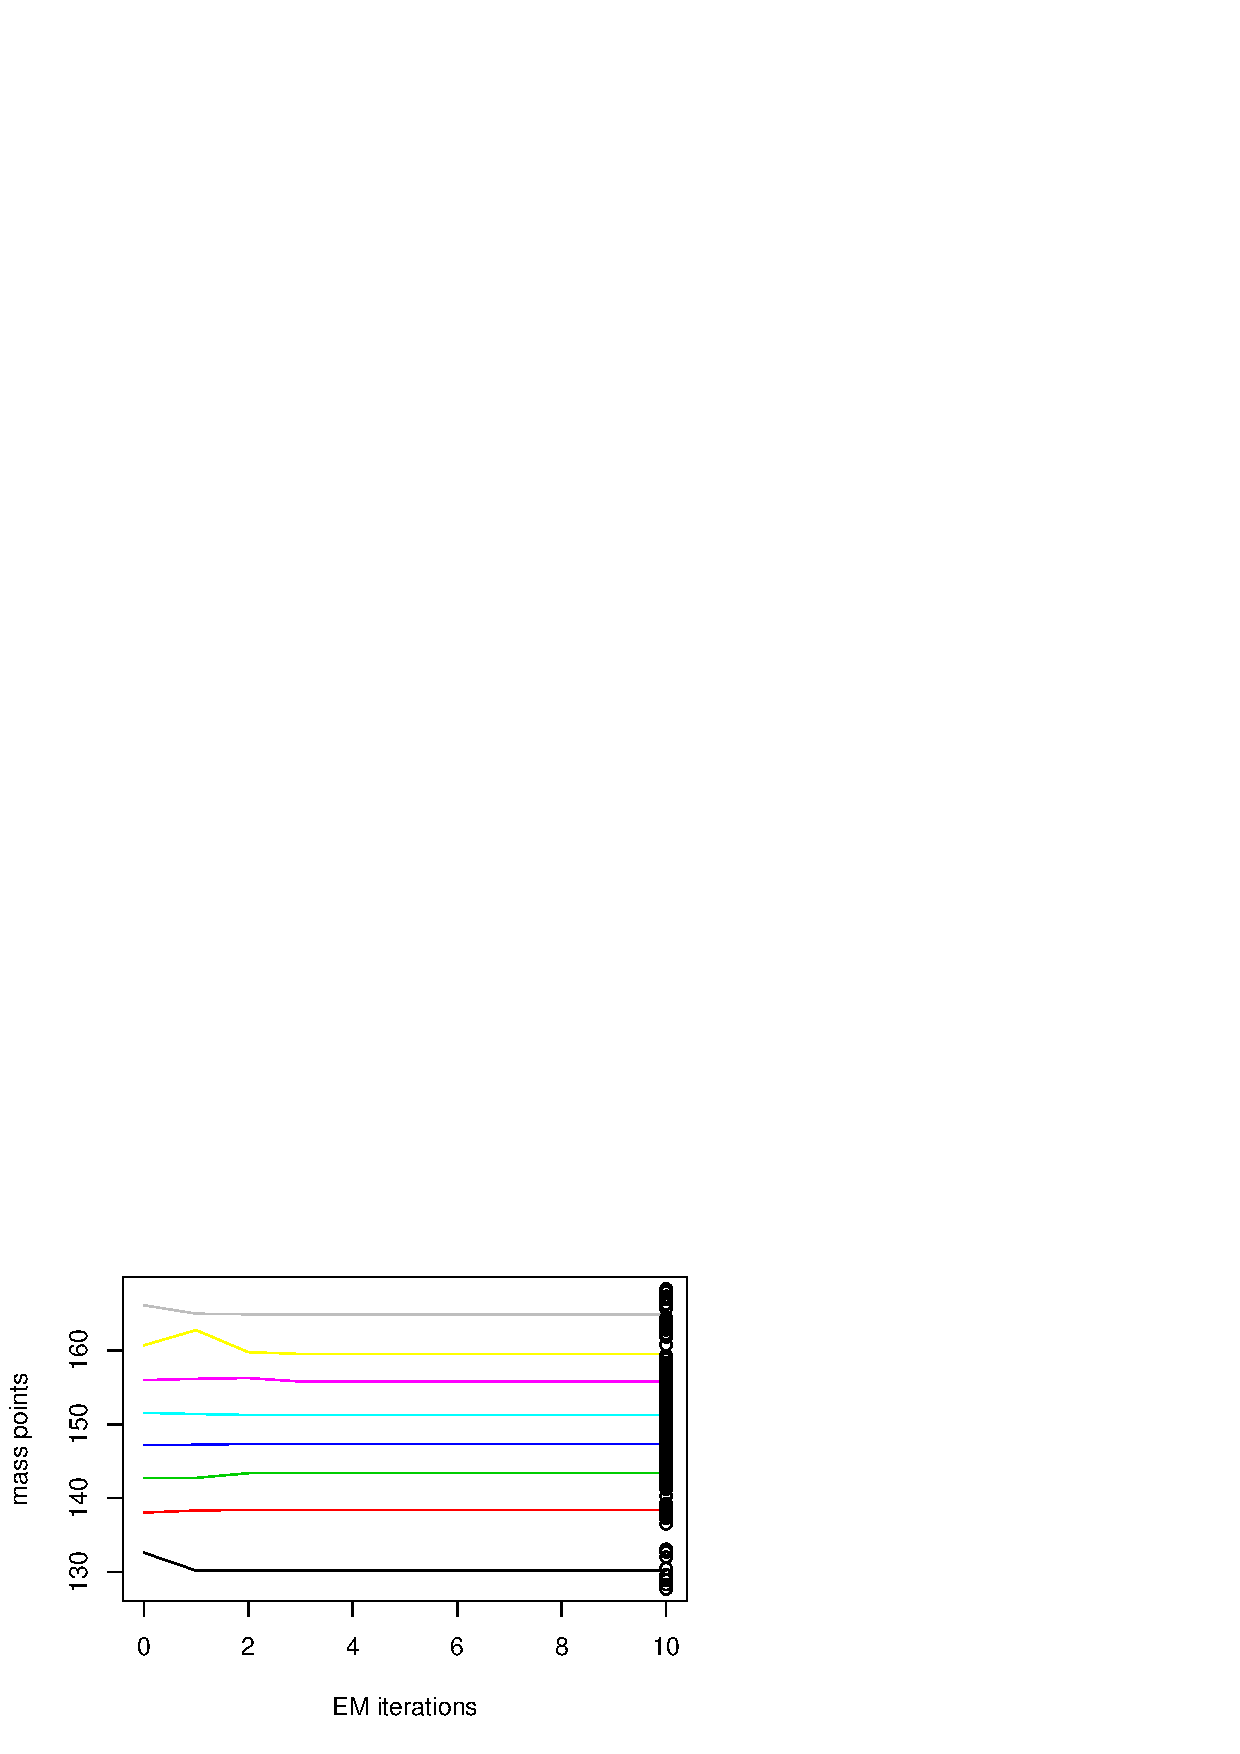
\includegraphics{npmlreg-v-042}
 
 Fig. 5: Convergence of EM for eight mass points, applied on Oxford boys data. 
 \end{minipage}
 
 
 
 
 \subsection{Spatial random effect models: Irish Suicide Data}
 
 
 The data considered here, available in the package {\bf npmlreg} via
 %39
\begin{Schunk}
\begin{Sinput}
> data(irlsuicide)
\end{Sinput}
\end{Schunk}
 describe the mortality due to suicide and intentional self-harm in the Republic of Ireland from 1989--1998.  
 Suicide rates are modelled using 
either the average crude rate or the relative risk as model parameter. The analysis of these data involves  a variance component model 
with regions as cluster variable, categorical covariates for gender and age, interaction terms, 
  and an offset representing the cluster sizes. The R code can be found in the {\tt Examples} section of the help file for {\tt allvc} (page 8 in the reference manual). 
While the random effect accounts for within-region correlation, it is worthwile to consider between-region correlation in this application.
Spatial correlation between regions is included 
 into the model by employing  an extra - fixed or random - covariate representing the average crude 
 suicide rates from the neighboring regions (or the average neighboring 
 standard mortality ratios, respectively). For details, see Sofroniou, Einbeck and Hinde (2006).
 
 
 \section{Citation}

The correct citation for R package {\bf npmlreg} can be queried with
%40
\begin{Schunk}
\begin{Sinput}
> citation(package = "npmlreg")
\end{Sinput}
\begin{Soutput}
To cite package ‘npmlreg’ in publications use:

  Jochen Einbeck, Ross Darnell and John Hinde (2007). npmlreg:
  Nonparametric maximum likelihood estimation for random effect models.
  R package version 0.43.

A BibTeX entry for LaTeX users is

  @Manual{,
    title = {npmlreg: Nonparametric maximum likelihood estimation for random effect
models},
    author = {Jochen Einbeck and Ross Darnell and John Hinde},
    year = {2007},
    note = {R package version 0.43},
  }

ATTENTION: This citation information has been auto-generated from the
package DESCRIPTION file and may need manual editing, see
‘help("citation")’ .
\end{Soutput}
\end{Schunk}
\medskip

\noindent The correct citation for this R vignette is 
\medskip
 
\noindent
\begin{description}
\item[EINBECK, J. and HINDE, J.] (2007). Nonparametric maximum
     likelihood estimation for random effect models in R. Vignette to R
     package  {\bf npmlreg} version 0.43.
\end{description} 
 
\section*{Acknowledgments}
 
The work on this R package was supported by Science
Foundation Ireland Basic Research Grant 04/BR/M0051.
  
\section{References}
 
 \begin{description}
 \item[AITCHISON, J. and AITKEN, C. G. G.] (1976).
Multivariate binary discrimination by kernel method.
{\em Biometrika} {\bf 63}, 413-420.
 \item [AITKIN, M.] (1996a). A general maximum likelihood
analysis of overdispersion in generalized linear models.  {\em
Statistics and Computing} {\bf 6}, 251--262.
\item[AITKIN, M.](1996b). Empirical Bayes shrinkage using
posterior random effect means from nonparametric maximum likelihood
estimation in general random effect models. {\em Statistical
Modelling:  Proceedings of the 11th IWSM 1996}, 87--94.
\item[AITKIN, M.] (1999). A general maximum likelihood analysis of variance components 
in generalized linear models.  {\em Biometrics}  {\bf 55} , 117--128.
\item[AITKIN, M. and FRANCIS, B.] (1995). 
Fitting Overdispersed Generalized Linear Models by Nonparametric Maximum Likelihood.
{\em GLIM Newsletter} {\bf 25 }, 37--45.
\item[AITKIN, M.] (2001). Likelihood and
Bayesian analysis of mixtures. {\em Statistical Modelling} {\bf
1}, 287--304.
\item[AITKIN, M., FRANCIS, B. and HINDE, J. ] (2005). 
{\em Statistical Modelling in GLIM 4} (2nd edition). Oxford, UK.  
\item[EINBECK, J. and HINDE, J.] (2006).
A note on NPML estimation for exponential family regression models with unspecified dispersion parameter.
{\em Austrian Journal of Statistics} {\bf 35}, 233--243. 
\item[EINBECK, J., HINDE, J. and DARNELL, R.] (2007).
A new package for fitting random effect models -- The npmlreg package.  {\em R News} {\bf 7}, 26--30. 
\item[EFRON, B.] (1986). Double exponential families and their use in generalized linear regression.
{\em JASA} {\bf 81}, 709--721.
\item[GOLDSTEIN, H.] (2003). {\em  Multilevel statistical models} (3rd edition). Arnold, London, UK.
\item[HINDE, J. ] (1982).
Compound Poisson Regression Models.
{\em Lecture Notes in Statistics} {\bf 14}, 109--121.
\item[LAIRD, N. M. ] (1978). Nonparametric maximum likelihood estimation of a mixing distribution. {\em JASA}, {\bf 73}, 805--811.
\item[POSTMAN, M., HUCHRA, J. P. and GELLER, M. J.] (1986). Probes of large-scale structures 
in the Corona Borealis region. {\em Astronomical Journal} {\bf 92},1238--1247.
\item[ROSNER, B.] (2000). {\em Fundamentals of
Biostatistics.} Thomson Learning, Duxbury, CA, USA.
\item[SOFRONIOU, N., EINBECK, J. and HINDE, J.] (2006). Analyzing Irish Suicide Rate with Mixture Models.
 In {\em Proceedings of the 21st International Workshop on Statistical Modelling, 3-7/07/06, Galway, Ireland}, 474--481.
\end{description}
\newpage






\section{Appendix: R Documentation}

A printed version of the help files is available in the reference manual, which can be downloaded from CRAN at

\begin{center}
{\tt http://cran.r-project.org/src/contrib/Descriptions/npmlreg.html}.
\end{center}

A list of all functions currently availabe in {\bf npmlreg} is given below:

%39
\begin{Schunk}
\begin{Sinput}
> ls("package:npmlreg")
\end{Sinput}
\begin{Soutput}
 [1] "alldist"               "allvc"                 "binomial.expand"      
 [4] "dkern"                 "expand"                "expand.vc"            
 [7] "family.glmmGQ"         "family.glmmNPML"       "gqz"                  
[10] "model.matrix.glmmGQ"   "model.matrix.glmmNPML" "plot.glmmGQ"          
[13] "plot.glmmNPML"         "post"                  "predict.glmmGQ"       
[16] "predict.glmmNPML"      "print.glmmGQ"          "print.glmmNPML"       
[19] "summary.glmmGQ"        "summary.glmmNPML"      "tolfind"              
[22] "weightslogl.calc.w"   
\end{Soutput}
\end{Schunk}

In addition, the data sets \texttt{irlsucide}, \texttt{hosp}, and \texttt{missouri} are available.
\end{landscape}
\end{document}
